\chapter{Mise en Œuvre du Sprint 1 : Développement et Déploiement de l'Infrastructure d'Analyse de Sentiments}

\section{Introduction}

Dans le cadre du sprint 1, l'équipe s'est concentrée sur le développement initial de l'infrastructure d'analyse de sentiments ainsi que sur son déploiement pour les premiers tests et évaluations. Ce sprint constitue la fondation technique de notre application d'analyse des commentaires d'Hespress. Voici un aperçu des activités réalisées durant cette période, qui ont permis d'établir les bases solides du système d'analyse automatisée.

L'objectif principal de ce premier sprint était de mettre en place l'architecture de base, d'intégrer les composants essentiels (FastAPI, Selenium, modèle de classification de sentiments) et de valider la faisabilité technique de la solution proposée. Cette approche itérative nous a permis de minimiser les risques techniques tout en garantissant une progression structurée du projet.

\section{Le Backlog du Sprint 1}

Le sprint 1 a été organisé autour de user stories prioritaires définies lors de l'analyse des besoins fonctionnels. Chaque user story a été accompagnée de critères d'acceptation clairs pour garantir la qualité et la conformité aux attentes.

\subsection{User Story 1.1 : Configuration de l'environnement de développement}

\textbf{En tant que} développeur \\
\textbf{Je veux} configurer l'infrastructure initiale de l'application d'analyse de sentiments \\
\textbf{Afin de} disposer d'une base solide sur laquelle construire le système complet

\textbf{Critères d'acceptation :}
\begin{itemize}
    \item L'environnement FastAPI est configuré et opérationnel
    \item La base de données est initialisée avec les schémas nécessaires
    \item Les dépendances du projet sont installées et documentées
    \item L'architecture microservices est mise en place avec Spring Gateway
\end{itemize}

\subsection{User Story 1.2 : Intégration du modèle d'analyse de sentiments}

\textbf{En tant que} développeur \\
\textbf{Je veux} intégrer le modèle cardiffnlp/twitter-xlm-roberta-base-sentiment \\
\textbf{Afin de} disposer d'un système de classification automatique des sentiments

\textbf{Critères d'acceptation :}
\begin{itemize}
    \item Le modèle est téléchargé et configuré dans l'environnement
    \item L'API de classification fonctionne avec des textes en arabe, français et darija
    \item Les scores de confiance sont retournés avec les prédictions
    \item Les performances de classification sont mesurées et documentées
\end{itemize}

\subsection{User Story 1.3 : Développement du module de web scraping}

\textbf{En tant qu'} utilisateur \\
\textbf{Je veux} collecter automatiquement les commentaires d'Hespress \\
\textbf{Afin de} disposer de données en temps réel pour l'analyse de sentiments

\textbf{Critères d'acceptation :}
\begin{itemize}
    \item Selenium est configuré pour naviguer sur le site Hespress
    \item Les commentaires sont extraits avec leurs métadonnées (date, article)
    \item Le système gère les mécanismes anti-bot et les limitations de taux
    \item Les données collectées sont stockées de manière structurée
\end{itemize}

\section{Benchmarking et Justification des Technologies Utilisées}

Le Sprint 1 a été consacré au développement et au déploiement de l'infrastructure d'analyse de sentiments en utilisant cardiffnlp/twitter-xlm-roberta-base-sentiment, FastAPI, Selenium et Spring Gateway.

\subsection{Choix Technologiques}

\subsubsection{Modèle cardiffnlp/twitter-xlm-roberta-base-sentiment}

Plusieurs modèles de classification de sentiments ont été évalués, notamment BERT, DistilBERT et XLM-RoBERTa. Le modèle cardiffnlp/twitter-xlm-roberta-base-sentiment a été choisi en raison de ses performances supérieures sur les textes multilingues et sa capacité à traiter les langues utilisées dans les commentaires marocains.

\textbf{Avantages :}
\begin{itemize}
    \item Support multilingue (arabe, français, darija)
    \item Performances optimisées pour les textes courts (commentaires)
    \item Pré-entraîné sur des données Twitter similaires aux commentaires web
    \item Architecture XLM-RoBERTa robuste et éprouvée
\end{itemize}

\subsubsection{FastAPI}

FastAPI a été choisi comme framework backend pour sa performance exceptionnelle et sa facilité d'intégration avec les modèles de machine learning. Il permet de créer des APIs RESTful rapidement tout en maintenant des performances élevées.

\textbf{Avantages :}
\begin{itemize}
    \item Performance élevée avec support asynchrone
    \item Documentation automatique avec OpenAPI/Swagger
    \item Validation automatique des données avec Pydantic
    \item Intégration native avec les bibliothèques ML Python
\end{itemize}

\subsubsection{Selenium WebDriver}

Selenium a été sélectionné pour le web scraping en raison de sa capacité à gérer les sites web dynamiques avec JavaScript, comme Hespress. Il permet une navigation réaliste et la gestion des éléments interactifs.

\textbf{Avantages :}
\begin{itemize}
    \item Gestion complète des sites web dynamiques
    \item Simulation du comportement utilisateur réel
    \item Support de différents navigateurs
    \item Gestion des mécanismes anti-bot avancés
\end{itemize}

\subsubsection{Spring Cloud Gateway}

Spring Gateway a été choisi comme API Gateway pour centraliser la gestion des requêtes et assurer la sécurité entre les microservices.

\textbf{Avantages :}
\begin{itemize}
    \item Routage intelligent des requêtes
    \item Load balancing automatique
    \item Sécurisation centralisée avec Keycloak
    \item Monitoring et métriques intégrés
\end{itemize}

\subsection{Justification des Choix}

Le choix de cette stack technologique répond à trois exigences importantes du projet :

\textbf{Scalabilité des ressources :} L'architecture microservices permet de faire évoluer indépendamment chaque composant selon les besoins de charge.

\textbf{Précision multilingue :} Le modèle XLM-RoBERTa assure une classification précise dans le contexte linguistique marocain complexe.

\textbf{Robustesse du scraping :} Selenium garantit une collecte fiable des données même avec les évolutions du site Hespress.

\subsection{Conclusion}

Le choix des technologies pour le Sprint 1 a été guidé par la recherche de solutions performantes, scalables et adaptées aux spécificités de l'analyse de sentiments dans le contexte marocain. Cette combinaison technologique constitue une base solide pour le développement d'un système d'analyse robuste et évolutif.

\section{Analyse et Conception}

\subsection{Description Textuelle}

Le développement du sprint 1 s'est articulé autour de plusieurs phases clés :

\textbf{Analyse des besoins techniques :} L'équipe a mené une analyse approfondie des contraintes techniques pour définir l'architecture optimale du système d'analyse de sentiments. Cela a inclus l'identification des composants critiques, des flux de données et des intégrations système nécessaires.

\textbf{Conception de l'architecture microservices :} Sur la base des besoins identifiés, l'architecture distribuée a été conçue, en déterminant les services principaux (collecte, analyse, stockage), les flux de communication et les mécanismes de sécurité. L'objectif était de garantir la scalabilité, la résilience et la facilité de maintenance.

\textbf{Développement des services de base :} Le développement initial s'est concentré sur la mise en place des services fondamentaux : API de classification, service de scraping, et gateway de routage. L'intégration avec le modèle de NLP et les sources de données a été prioritaire.

\textbf{Tests d'intégration :} Des tests d'intégration ont été mis en place pour valider le bon fonctionnement des interactions entre services. Cela a permis de détecter et corriger rapidement les problèmes de communication et de performance.

\textbf{Déploiement initial :} Une version initiale du système a été déployée sur un environnement de test pour permettre aux membres de l'équipe de l'évaluer et de fournir des retours d'expérience. Cela a également permis de commencer à collecter des données réelles pour valider l'efficacité du système.

\subsection{Diagramme de Cas d'Utilisation du Sprint 1}

\begin{figure}[H]
\centering
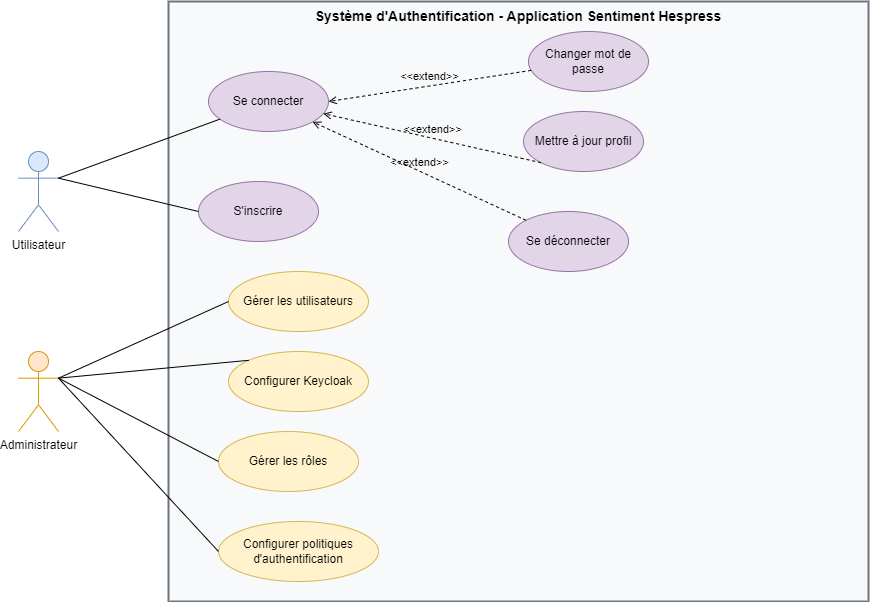
\includegraphics[width= 10 cm , height=10 cm]{assets/images/auth-usecase.png} 
\caption{Diagramme de cas d'utilisation du sprint 1}
\label{fig:sprint1-usecase}
\end{figure}

Ce diagramme illustre les interactions principales entre les acteurs (administrateur, analyste) et le système durant le premier sprint. Les cas d'utilisation se concentrent sur la configuration du système, la collecte de données et l'analyse de base des sentiments.

\subsection{Diagramme de Classe du Sprint 1}

\begin{figure}[H]
\centering
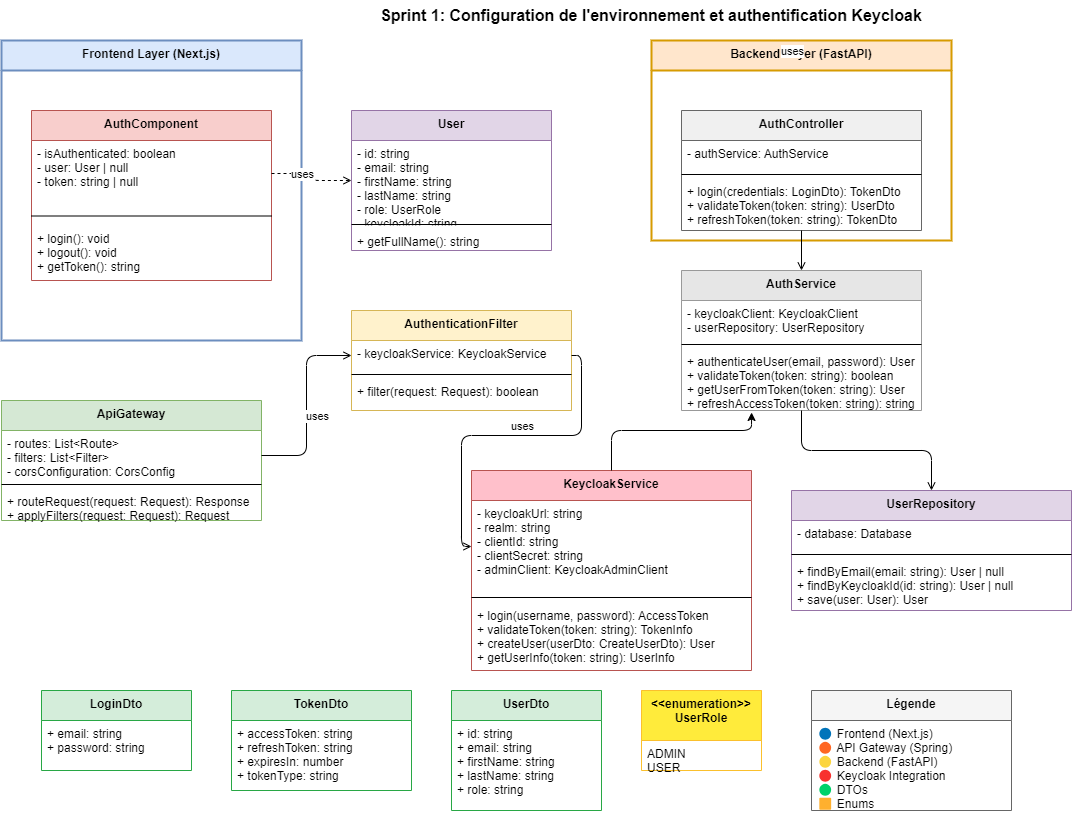
\includegraphics[width=0.9\textwidth]{assets/images/sprint1-class.png}
\caption{Diagramme de classe du sprint 1}
\label{fig:sprint1-class}
\end{figure}

L'architecture objet du sprint 1 met en évidence les classes principales : CommentScraper, SentimentAnalyzer, CommentModel, et AnalysisResult. Ces classes forment le cœur du système d'analyse de sentiments.

\subsection{Architecture de Classification de Sentiments}

\begin{figure}[H]
\centering
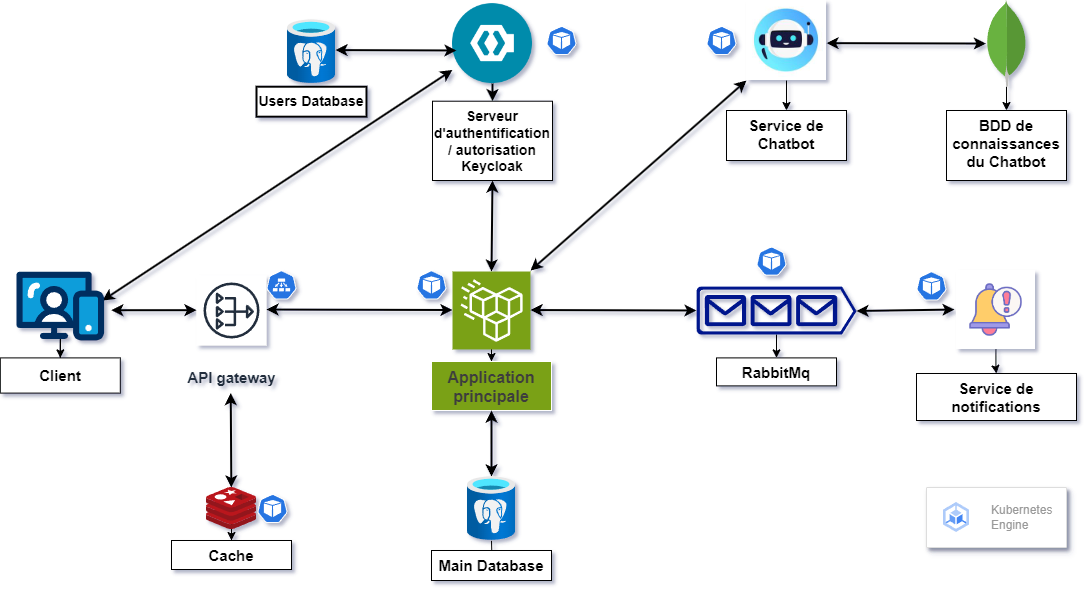
\includegraphics[width=0.8\textwidth]{assets/images/architecture.png}
\caption{Architecture du système d'analyse de sentiments}
\label{fig:sentiment-architecture}
\end{figure}

Le système d'analyse de sentiments utilise une approche en pipeline qui traite les commentaires depuis leur collecte jusqu'à la génération des insights analytiques. Le modèle XLM-RoBERTa constitue le cœur du processus de classification, permettant une analyse multilingue précise des sentiments exprimés dans les commentaires d'Hespress.

\subsection{Diagramme de Séquence du Sprint 1}

\begin{figure}[H]
\centering
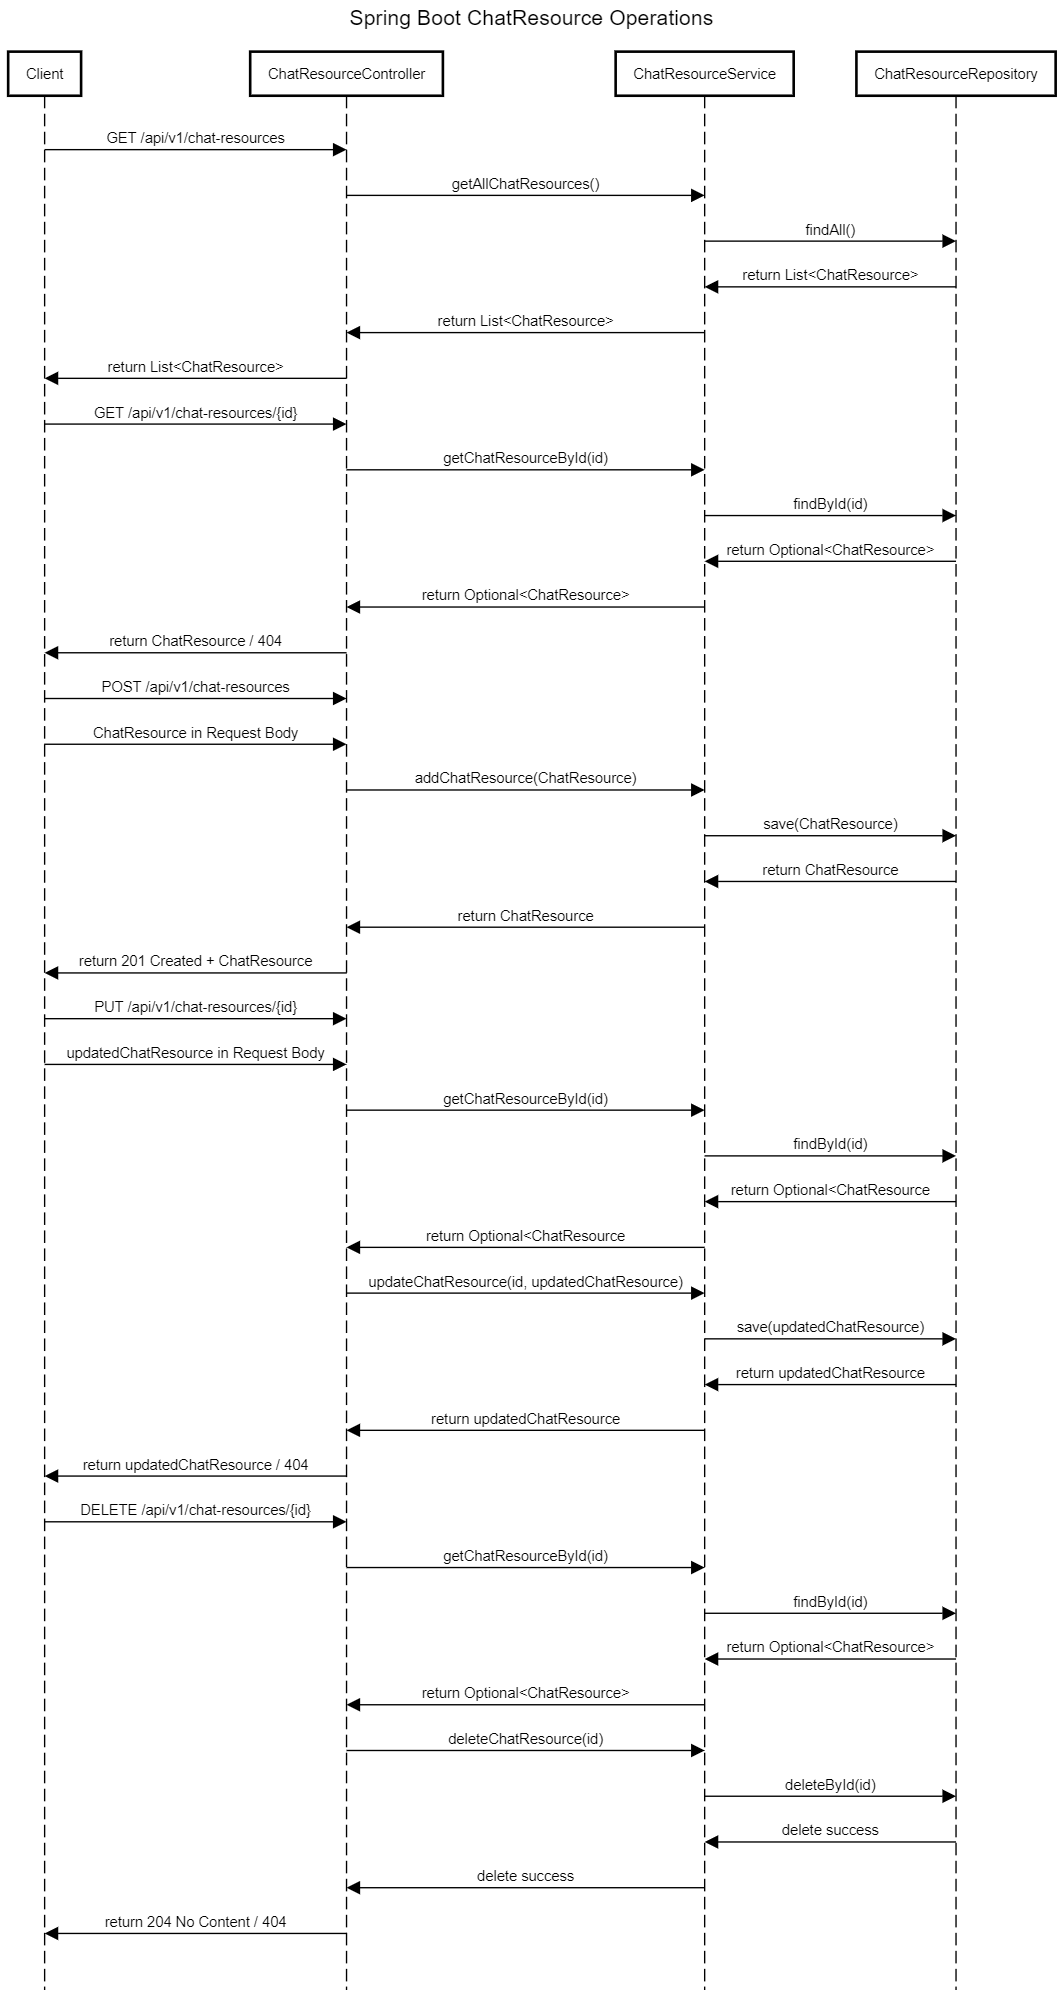
\includegraphics[width=0.9\textwidth]{assets/images/chat-res-seq.png}
\caption{Diagramme de séquence du processus d'analyse}
\label{fig:sprint1-sequence}
\end{figure}

Ce diagramme détaille le flux d'exécution depuis la requête de collecte jusqu'à la restitution des résultats d'analyse. Il montre l'orchestration entre les différents services et la gestion des données tout au long du pipeline de traitement.

\section{Réalisation du Sprint 1}

Le sprint 1 a abouti à la mise en place d'un système fonctionnel d'analyse de sentiments capable de collecter et analyser les commentaires d'Hespress. Les premières démonstrations ont validé la faisabilité technique et l'efficacité de l'approche choisie.

\subsection{Interface de Configuration}

L'interface développée permet aux administrateurs de configurer les paramètres de collecte et de lancer les processus d'analyse. L'ergonomie intuitive facilite la prise en main et la gestion quotidienne du système.

\subsection{Performances du Modèle}

Le modèle cardiffnlp/twitter-xlm-roberta-base-sentiment a démontré des performances satisfaisantes sur les premiers échantillons de commentaires, avec une précision particulièrement notable sur les textes en darija et en arabe marocain. Les résultats de classification montrent une bonne corrélation avec les évaluations manuelles effectuées par l'équipe.

\subsection{Collecte de Données}

Le système de scraping développé avec Selenium s'est montré robuste face aux mécanismes de protection d'Hespress. La collecte automatisée fonctionne de manière stable et respecte les bonnes pratiques d'éthique web.

\subsection{Validation et Perspectives}

Le sprint 1 a posé les bases solides du système d'analyse de sentiments, en validant les choix technologiques et en démontrant la faisabilité de la solution. Les retours d'expérience recueillis lors de cette phase sont précieux pour orienter les développements futurs et assurer le succès du projet.

Les prochains sprints se concentreront sur l'enrichissement des fonctionnalités d'analyse, l'amélioration de l'interface utilisateur et l'optimisation des performances pour traiter des volumes de données plus importants.